%%%describing the basic usage

This chapter deals with the basic interface provided by the layer 1 types
implemented in \libpniio. All types concerning Nexus reside in one of the
namespaces embedded in {\tt pni::io::nx}. The namespaces below this one 
indicate either a particular storage backend (currently only HDF5 is
implemented).

To use the Nexus part of the library just add 
\begin{cppcode}
#include <pni/io/nx/nx.hpp>
\end{cppcode}
to your source file. 

%%%===========================================================================
\section{Working with files}
\input{tex/nexus_files.tex}


%%%===========================================================================
\section{Working with groups}

\nexus\ groups are instances of the \nxgroup\ template. They can be considered
as containers for fields and other groups and expose an STL compliant interface. 
To start working with groups in a file one hast to first obtain the root group 
with 
\begin{cppcode}
h5::nxfile file = h5::nxfile::open_file("test.nxs");
h5::nxgroup root = file.root();
\end{cppcode}

\subsection{Creating groups}

New groups are created by means of the \cpp{create\_group} member function of
\nxgroup
\begin{cppcode}
h5::nxgroup entry = root.create_group("scan_1","NXentry");
\end{cppcode}
This method takes two arguments where the first one is mandatory and denotes the
name of the group while the second one is optional and determines the
\nexus-class of the group. If the last argument is omitted a simple HDF5 group
is created (without an \cpp{NX\_class}  attribute).

Like files, groups are automatically destroyed when an instance looses scope,
but they can also be deliberately closed using their \cpp{close()} method.

%%%===========================================================================
\subsection{Accessing children}

Access to the direct children of a group instance is given via the 
\cpp{at()} method or the \cpp{[]} operator. Both accept either a numeric index 
of a child or its name as an argument. To loop over all children of the 
root group the following code could be used
\begin{cppcode}
h5::nxfile f = ....;
h5::nxgroup root = f.root();

for(size_t i=0;i<root.size();++i) std::cout<<root[i].name()<<std::endl;
\end{cppcode}
As for STL containers, the \cpp{size()} method returns the number of children 
of a group. To access a particular group via its name one can use
\begin{cppcode}
h5::nxfile f = ....;
h5::nxgroup root = f.root();

h5::nxgroup entry = root["entry"]; //alternatively root.at("entry");
\end{cppcode}
Unlike for STL containers both access variants (\cpp{at()} or \cpp{[]}) will 
throw an exception if a particular child could not be found or the index passed
exceeds the total number of children of the group. In addition to this simple 
access interface \nxgroup\ also exposes a fully STL compliant iterator 
interface. However, in order to use it some more deeper knowledge about 
\libpniio\ is required and thus this topic will be dealt with in
Section~\ref{section:group_iteration}.

%%%===========================================================================
\subsection{Other group related member functions}

Like files, groups posses an \cpp{is\_valid()} method which allows checking the 
state of a group. Similar to files, default constructed instances of \nxgroup\
are not valid. 
\begin{cppcode}
h5::nxgroup entry; 

if(!entry.is_valid()) std::cerr<<"The entry group is not valid!"<<std::endl;
\end{cppcode}
The getter methods \cpp{name()} and \cpp{filename()} return the name of the
group and the name of the file the group is stored in respectively.
Finally the \cpp{parent()} function returns the parent group of the a group.
In order to use the \cpp{parent()} member function a bit more extra care is 
used. When using the method in a simple way like 
\begin{cppcode}
h5::nxgroup p = other_group.parent();
\end{cppcode}
everything will be fine. However, when we want to use the return value of 
\cpp{parent()} as a temporary we have to do an explicit conversion to 
\cpp{nxgroup} like this
\begin{cppcode}
std::cout<<h5::nxgroup(entry_group.parent())<<std::endl;
\end{cppcode}
The reason for this is that \cpp{parent()} does not really return an 
instance of \cpp{nxgroup} but rather of \cpp{nxobject}. 
But \nxobject\ can be converted to \nxgroup\ safely. The reason 
for this behavior will be explained in detail in Section~\ref{section:nxobject}.




%%%===========================================================================
\section{Working with fields}

Fields are the basic data holding facilities in \libpniio\ and are represented
by instances of \nxfield. One can imagine a field as a multidimensional array 
stored on disk. Thus, it has quite similar properties than instances of 
\cpp{mdarray} in \libpnicore.  It is impossible to create a purely 
scalar field with \libpniio\ as every field should be extensible if required. 

%%%===========================================================================
\subsection{Creating fields}

Fields are created as children of a particular group instance. Creating fields
is a rather complex task as there are many options available so lets start with 
the simplest possible example
\begin{cppcode}
h5::nxgroup entry = root["entry"];
h5::nxfield field = entry.create_field<float32>("temperature");
\end{cppcode}
This creates a 1D field with a single element. This is as closest one can get 
to store a scalar value. The template parameter of the \cpp{create\_field}
method can be any type supported by \libpnicore.  For multidimensional fields
use 
\begin{cppcode}
h5::nxgroup entry = root["entry"];
h5::nxfield field = entry.create_field<float32>("temperature",shape_t{3,4});
\end{cppcode}
which will create a $2$-dimensional field with a shape of $(3,4)$ and a total
size of $12$ elements.
When using HDF5 as a storage format a compression algorithm can be associated
with a field. This algorithm will later on be used to compress the data stored
in a field and thus reduce disk utilization of the file. 
Currently only the standard deflate filter is supported 
\begin{cppcode}
h5::nxgroup entry = root["entry"];
h5::nxdeflate_filter deflate(4,false);
h5::nxfield field = entry.create_field<float32>("temperature",shape_t{3,4},deflate);
\end{cppcode}
In this particular case the filter uses a compression level of $4$ and no 
fletcher pre-sorting of the data. 

%%%===========================================================================
\subsection{Reading and writing data}

Fields provide two basic methods for reading and writing data: \cpp{read()} and
\cpp{write()}. Both member functions accept a single argument which can be an
instance of the following types
\begin{center}
    \begin{tabular}{l|p{0.6\linewidth}}
        {\bf type} & {\bf description} \\
        \hline
        \hline
        {\tt mdarray<...>} & an instance of the {\tt mdarray} template \\
        \hline
        {\tt array} & an instance of the array type erasure \\
        \hline
        {\tt T\& } & a single scalar value of the fields element type or a 
        convertible type \\
        \hline
    \end{tabular}
\end{center}
In addition there is a special version of \cpp{read()} and \cpp{write()}
available for legacy code with raw pointers. The two functions have the
signatures
\begin{cppcode}
template<typename T> void read(size_t n,T *ptr);
template<typename T> void write(size_t n,const T *ptr);
\end{cppcode}
The additional first argument \cpp{n} is the number of elements of type \cpp{T}
referenced by the pointer \cpp{*ptr}. This number ensures that the functions 
can check if the size of the field matches the number of elements which should
be read from or written to memory.
A scalar can be read from a field simply with
\begin{cppcode}
float32 temperature; 
h5::nxfield field = ...;
field.read(temperature);
\end{cppcode}
and writing runs exactly as one would expect
\begin{cppcode}
float32 temperator = ...;
h5::nxfield field = ...;
field.write(temperature);
\end{cppcode}
The same simple concept applies to all other types. For an instance of 
\cpp{mdarray} the code would look like this
\begin{cppcode}
auto data = dynamic_array<uint32>::create(shape_t{1024,1024});
h5::nxfield background = ....;

background.write(data); //writing

background.read(data);  //reading
\end{cppcode}

The \cpp{read()} and \cpp{write()} member functions perform a size check on
their arguments. The size of the argument must match the size of the field. 
In the case of scalar data a field-size of $1$ is assumed. If argument and field
size do not match a \cpp{size\_mismatch\_exception} is thrown.

%%%===========================================================================
\subsection{Growing fields}

\begin{figure}
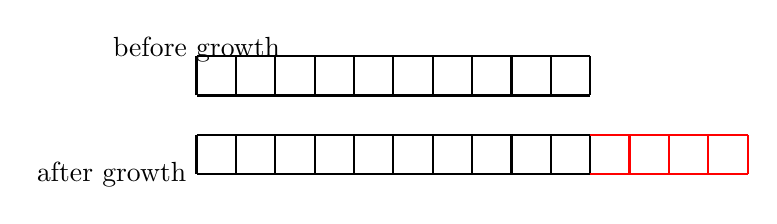
\begin{tikzpicture} [field/.style = {thick,step=5mm} ]
\draw[field] (0mm,0mm) node[anchor = east,above=3mm] {before growth} grid (50mm,5mm); 
\draw[field] (0mm,-10mm) node[anchor=east] {after growth} grid +(50mm,5mm);
\draw[field,color=red] (50mm,-10mm)  grid +(20mm,5mm);
\end{tikzpicture}
\end{figure}

The reason why there are no purely scalar fields is that during an experiment 
one would append data to a field as the measurement progresses. 
For this purpose \nxfield\ provides a \cpp{grow()} method which allows to 
extend the field along a particular dimension. The member function has the 
signature
\begin{cppcode}
void grow(size_t e,size_t n=1)
\end{cppcode}
where the first (mandatory) argument is the index of the dimension along which
the field should grow and the second (optional) argument contains the number of 
elements by which to grow. 

%%%===========================================================================
\subsection{Partial reading and writing}

Nexus fields support partial IO with the {\tt ()} operator which applies
selections to the field instances. 
\begin{cppcode}
h5::nxfield spectra = ...;

auto s = spectra.shape<shape_t>();

auto spectrum = dynamic_array<uint32>::create(shape_t{s[1]});

for(size_t i=0;i<s[0];++i)
{
    spectra(i,slice(0,s[1])).read(spectrum);
    .... process data ...
}
\end{cppcode}
The selection mechanism works the same as for the {\tt mdarray} template. 

%%%===========================================================================
\subsection{Field inquiry}



%%%===========================================================================
\section{Working with attributes}



